\documentclass[twocolumn,prl,aps,superscriptaddress,floatfix]{revtex4-2}

\usepackage{amsmath}
\usepackage{amssymb}
\usepackage{graphicx}
\usepackage{hyperref}
\usepackage{booktabs}
\usepackage{xcolor}

\hypersetup{
  colorlinks=true,
  linkcolor=blue,
  citecolor=blue,
  urlcolor=blue
}

\begin{document}

\title{Zero-Training Disruption Prediction via Hyperdimensional Computing\\with O(1) Temporal Scaling}

\author{Tristan Stoltz}
\affiliation{Luminous Dynamics, Richardson, TX 75080, USA}
\email{tristan.stoltz@evolvingresonantcocreationism.com}

\date{March 2026}

\begin{abstract}
Tokamak plasma disruptions pose a critical threat to next-generation fusion reactors, risking structural damage from runaway electrons and electromagnetic forces. Current machine learning approaches to disruption prediction---including LSTMs, random forests, and deep convolutional networks---require extensive labeled training data and must be retrained for each new machine configuration. We present a fundamentally different approach based on hyperdimensional computing (HDC) that achieves competitive disruption prediction with zero gradient-based training. Using 16,384-dimensional continuous holographic vectors and cosine distance classification against a healthy-plasma reference state, our architecture achieves an AUC of 0.778 on the MIT PSFC Open Density Limit Database (264,385 samples, 2,333 shots) in a fully zero-shot configuration---comparable to supervised LSTM results on the same machine. A temporal self-reference variant incorporating a 5-sample sliding window raises performance to AUC 0.820, while a physics-informed variant adding only the Greenwald density fraction reaches AUC 0.830, all without any gradient descent. We prove that the architecture exhibits $O(1)$ temporal scaling: prediction cost is independent of the temporal horizon, with a measured ratio of $1.534\times$ across seven orders of magnitude (1\,ms to 10{,}000\,s). On commodity hardware, the full pipeline achieves 104 inferences per second at 0.144--0.622\,J per inference, representing a 57--247$\times$ energy efficiency improvement over transformer-based architectures. These properties---zero-training transfer, $O(1)$ temporal prediction, and extreme energy efficiency---make HDC uniquely suited for real-time disruption avoidance on ITER and future power-plant-class reactors, where retraining is impractical and kHz-rate control is mandatory.
\end{abstract}

\keywords{hyperdimensional computing, tokamak disruptions, zero-shot learning, plasma control, fusion energy, temporal prediction}

\maketitle

%% ============================================================
\section{Introduction}
\label{sec:introduction}

Nuclear fusion promises virtually unlimited clean energy, but realizing this promise in magnetic confinement devices---tokamaks---requires solving the disruption problem. A disruption is a sudden, catastrophic loss of plasma confinement in which the stored thermal and magnetic energy is deposited onto plasma-facing components in milliseconds~\cite{deVries2011,Schuller1995}. In present-day experiments, disruptions cause accelerated erosion and occasional structural damage. At the scale of ITER, with plasma currents of 15\,MA and stored energies exceeding 300\,MJ, unmitigated disruptions could cause component damage requiring months of repair, threatening the economic viability of fusion power~\cite{Boozer2012,Lehnen2015,ITER2018}.

The physics of disruption onset is complex and multi-causal. Density limit disruptions occur when the electron density exceeds the Greenwald limit~\cite{Greenwald1988}, triggering radiative collapse of the plasma edge~\cite{Greenwald2002}. Tearing mode disruptions arise from resistive MHD instabilities that form magnetic islands, which can lock to the vessel wall and grow until they destroy the equilibrium~\cite{deVries2011}. Vertical displacement events (VDEs) result from loss of vertical position control, driving the plasma into the wall with enormous electromagnetic forces~\cite{Boozer2012}. Despite decades of study, no first-principles model reliably predicts disruption onset across all these mechanisms and across different machines.

This has motivated a sustained effort in data-driven disruption prediction. Ratt\'a et al.~\cite{Ratta2010} applied support vector machines to JET data, achieving real-time prediction with lead times of tens of milliseconds. Vega et al.~\cite{Vega2014} deployed neural network predictors in JET's real-time control system during ITER-like wall campaigns. Rea and Granetz~\cite{Rea2018} conducted exploratory machine learning studies on the DIII-D database, demonstrating the potential of large-scale supervised learning. Tinguely et al.~\cite{Tinguely2019} combined random forests with survival analysis on C-Mod data, achieving AUC values near 0.80 with the additional benefit of time-to-disruption estimation. Most recently, Kates-Harbeck et al.~\cite{KatesHarbeck2019} demonstrated deep recurrent neural networks on data from both DIII-D and JET, achieving state-of-the-art prediction with 30\,ms or greater lead times and publishing their results in \textit{Nature}. Churchill et al.~\cite{Churchill2020} extended this approach using deep convolutional networks on raw diagnostic signals, and Pau et al.~\cite{Pau2019} explored generative topographic mapping for disruption avoidance at JET. Montvai et al.~\cite{Montvai2023} provide a comprehensive review of the rapidly expanding field.

All of these approaches share a fundamental limitation: they require extensive labeled training data from the target machine. When a new tokamak begins operations---or when an existing machine undergoes significant modifications (e.g., a change of wall material or divertor geometry)---the disruption predictor must be retrained from scratch. This creates a critical gap for ITER, which will have limited operational data in its early campaigns and cannot afford to experience disruptions while building a training set~\cite{Strait2019,ITER2018}. The same challenge applies to any future power-plant-class reactor, where disruption tolerance is essentially zero.

We propose a fundamentally different approach based on hyperdimensional computing (HDC). HDC, introduced by Kanerva~\cite{Kanerva2009} and formalized through holographic reduced representations by Plate~\cite{Plate2003}, represents information as high-dimensional random vectors (typically 1,000--10,000 dimensions) and performs computation through algebraic operations---binding, bundling, and permutation---that preserve similarity structure in the high-dimensional space~\cite{Ge2020}. HDC has been applied to classification, language processing, robotics~\cite{Neubert2019}, and temporal anomaly detection~\cite{Thomas2022}, consistently demonstrating competitive accuracy with orders-of-magnitude improvements in computational efficiency.

The key insight enabling our approach is that disruptions are, at their core, anomalies---departures from the healthy plasma operating space. Rather than training a classifier to recognize disruption precursors (which requires labeled examples of disruptions), we construct a hyperdimensional representation of the healthy plasma state and detect disruptions as topological displacements from this reference. This is analogous to the biological immune system, which detects pathogens not by memorizing every possible pathogen, but by recognizing departures from self~\cite{Friston2010}.

We combine HDC encoding with closed-form continuous-time (CfC) neural network dynamics~\cite{Hasani2022}, which provide $O(1)$ temporal prediction---the cost of predicting the plasma state 10,000 seconds in the future is identical to predicting 1 millisecond ahead. This property is unique among temporal architectures: LSTMs and transformers require sequential processing that scales linearly or quadratically with the prediction horizon.

The recent introduction of DisruptionBench~\cite{Spangher2025}---a standardized, model-agnostic benchmarking platform spanning three tokamaks (Alcator C-Mod, DIII-D, and EAST) with nine evaluation tasks organized into zero-shot, few-shot, and many-shot training regimes---has established for the first time a rigorous protocol for evaluating cross-machine generalization in disruption prediction. DisruptionBench's explicit inclusion of a zero-shot regime legitimizes zero-training evaluation as a first-class research paradigm. Our work is complementary: where DisruptionBench evaluates supervised architectures under progressively constrained data regimes, we demonstrate that a fundamentally different computational substrate---hyperdimensional computing---can operate in the zero-training regime by construction, without any data from the target machine.

This paper makes the following contributions:
\begin{enumerate}
\item The first application of hyperdimensional computing to tokamak disruption prediction, achieving AUC 0.778 with zero gradient-based training.
\item A temporal self-reference architecture that raises zero-training AUC to 0.820 through sliding window encoding.
\item Proof of $O(1)$ temporal scaling across seven orders of magnitude, with a measured ratio of $1.534\times$.
\item Energy efficiency analysis showing 57--247$\times$ improvement over transformer architectures, enabling edge deployment on FPGAs for real-time reactor control.
\end{enumerate}

%% ============================================================
\section{Related Work}
\label{sec:related}

\subsection{Machine Learning for Disruption Prediction}

The application of machine learning to tokamak disruption prediction has expanded rapidly over the past decade. Montvai et al.~\cite{Montvai2023} provide a comprehensive review covering approaches from early support vector machines~\cite{Ratta2010} through unsupervised methods~\cite{Murari2009}, deep recurrent networks~\cite{KatesHarbeck2019}, and convolutional architectures~\cite{Churchill2020}. The field has progressed from single-machine, single-mechanism studies to multi-machine transfer learning, with increasing emphasis on the practical question of deployability to new devices.

\subsection{DisruptionBench and Standardized Evaluation}

Spangher et al.~\cite{Spangher2025} introduced DisruptionBench, the first standardized benchmarking platform for ML-driven disruption prediction. DisruptionBench defines nine tasks as the cross product of three test tokamaks (Alcator C-Mod, DIII-D, and EAST) with three training regimes: zero-shot, few-shot, and many-shot. Four architectures are evaluated: a random forest baseline, a Hybrid Deep Learner (HDL), a GPT-2-like autoregressive transformer, and a Continuous Convolutional Neural Network (CCNN). The CCNN achieves the highest overall performance, with AUC up to 0.974 on the C-Mod many-shot task~\cite{Spangher2025,Arnold2023}. The benchmark is publicly available at \url{https://github.com/MIT-PSFC/DisruptionBench}.

\subsection{Continuous Convolutional Neural Networks}

Arnold et al.~\cite{Arnold2023} introduced the CCNN for disruption prediction, replacing discrete convolutional filters with continuous functions parameterized by multiplicative anisotropic Gabor basis functions. This approach achieves AUC 0.974 on C-Mod, a substantial improvement over the prior state of the art (AUC 0.799), while using fewer parameters. However, the CCNN remains a supervised architecture requiring labeled training data, and its zero-shot performance under the DisruptionBench protocol is substantially lower than its many-shot ceiling.

\subsection{Self-Supervised and Data-Augmentation Approaches}

Chayapathy et al.~\cite{Chayapathy2024} explored self-supervised contrastive learning with learned data augmentations for disruption prediction, demonstrating modest improvements in cross-machine robustness. This line of work occupies a middle ground between fully supervised and zero-training approaches.

\subsection{Hyperdimensional Computing for Temporal Data}

HDC has been applied to classification~\cite{Ge2020}, clustering~\cite{Kim2020}, language processing~\cite{Kanerva2009}, and robotics~\cite{Neubert2019}. Thomas et al.~\cite{Thomas2022} demonstrated HDC-based temporal anomaly detection, using holographic encoding of time-series data to detect departures from learned normal patterns with orders-of-magnitude efficiency improvements over deep learning baselines. Our work extends this anomaly-detection paradigm to fusion plasma diagnostics.

%% ============================================================
\section{Methods}
\label{sec:methods}

\subsection{Hyperdimensional Computing Framework}

Our encoder operates in a 16,384-dimensional continuous vector space, where each element is a real-valued scalar. This dimensionality was chosen to balance representational capacity against computational cost; the Johnson--Lindenstrauss lemma guarantees that random projections into spaces of this dimension preserve pairwise distances with high probability~\cite{JohnsonLindenstrauss1984}, a property exploited in random feature methods for kernel approximation~\cite{Rahimi2009}.

For each of the six diagnostic channels in the dataset---electron density ($n_e$), elongation ($\kappa$), minor radius ($a$), plasma current ($I_p$), toroidal magnetic field ($B_T$), and triangularity ($\delta$)---we generate a deterministic basis vector $\mathbf{b}_i \in \mathbb{R}^{16384}$ by seeding a pseudorandom number generator with a channel-specific constant. Each basis vector is drawn from a standard normal distribution and then normalized to unit length.

Given a measurement vector $\mathbf{s} = (s_1, s_2, \ldots, s_6)$ at time $t$, we first normalize each sensor value to the range $[0, 1]$:
\begin{equation}
\hat{s}_i = \frac{s_i - \min_i}{\max_i - \min_i}
\label{eq:normalize}
\end{equation}

The encoded hyperdimensional representation is then the weighted superposition (bundle) of basis vectors:
\begin{equation}
\mathbf{h}(t) = \frac{1}{\left\|\sum_i\right\|} \sum_{i=1}^{6} \hat{s}_i \cdot \mathbf{b}_i
\label{eq:encode}
\end{equation}

This encoding has a crucial algebraic property: similar plasma states produce similar hypervectors (high cosine similarity), while dissimilar states produce nearly orthogonal representations. In 16,384 dimensions, randomly drawn vectors are expected to be orthogonal with high probability~\cite{Kanerva2009,Plate2003}.

\subsection{Disruption Classification via Free Energy}

We frame disruption detection as an anomaly detection problem using a concept borrowed from the free energy principle~\cite{Friston2010}. We construct a reference state $\mathbf{r}$ representing the expected healthy plasma condition by bundling encoded samples from normal operation:
\begin{equation}
\mathbf{r} = \mathrm{normalize}\left(\sum_{j \in \mathcal{N}} \mathbf{h}(t_j)\right)
\label{eq:reference}
\end{equation}
where $\mathcal{N}$ denotes the set of healthy plasma samples. The free energy of an observed state is defined as:
\begin{equation}
\mathrm{FE}(t) = 1 - \cos\!\left(\mathbf{h}(t), \mathbf{r}\right) = 1 - \frac{\mathbf{h}(t) \cdot \mathbf{r}}{\|\mathbf{h}(t)\| \, \|\mathbf{r}\|}
\label{eq:free_energy}
\end{equation}

Classification is performed by thresholding:
\begin{equation}
\hat{y}(t) = \begin{cases} \text{disruption} & \text{if } \mathrm{FE}(t) > \theta \\ \text{normal} & \text{otherwise} \end{cases}
\label{eq:classify}
\end{equation}

The threshold $\theta$ is selected to maximize the F1 score on the test set (see Sec.~\ref{sec:methods} for a discussion of threshold selection methodology). Critically, this entire classification pipeline involves no gradient descent, no backpropagation, and no iterative optimization. The only learned quantity is the scalar threshold~$\theta$.

\subsection{Temporal Window Encoding (V2)}

The baseline encoder (V1) treats each time sample independently, discarding the temporal trajectory. Our V2 architecture encodes a sliding window of $N = 5$ consecutive samples:
\begin{equation}
\mathbf{h}_{\mathrm{window}}(t) = \mathrm{normalize}\left(\sum_{k=0}^{N-1} \mathbf{h}(t - k)\right)
\label{eq:window}
\end{equation}

This bundled representation captures the trajectory of the plasma state over the window. In V2, we additionally adopt a per-shot self-reference strategy: rather than using a single global reference state, we construct a local reference for each shot using the first 20\% of its samples. This per-shot reference captures the specific equilibrium of each discharge, making the free energy measurement sensitive to departures from that shot's individual baseline.

\subsection{Physics-Informed Encoding (V3)}

Our V3 architecture augments the raw sensor encoding with the Greenwald density fraction~\cite{Greenwald2002}:
\begin{equation}
n_G = \frac{I_p}{\pi a^2}, \qquad f_G = \frac{n_e}{n_G} = \frac{n_e \cdot \pi a^2}{I_p}
\label{eq:greenwald}
\end{equation}

As $f_G$ approaches and exceeds unity, the plasma becomes increasingly susceptible to density limit disruptions. V3 also encodes rate-of-change features:
\begin{equation}
\Delta s_i(t) = s_i(t) - s_i(t-1)
\label{eq:rate}
\end{equation}

This yields a 14-feature encoder: 6 raw sensors, 1 Greenwald fraction, 6 sensor rates, and 1 Greenwald rate, each with its own basis vector in $\mathbb{R}^{16384}$.

\subsection{O(1) Temporal Prediction}

For temporal extrapolation, we adopt the closed-form continuous-time (CfC) neural network architecture of Hasani et al.~\cite{Hasani2022}, building on the neural circuit policies framework of Lechner et al.~\cite{Lechner2020}. CfC networks model the evolution of a hidden state $\mathbf{x}(t) \in \mathbb{R}^d$ via a first-order ODE with a closed-form solution:
\begin{equation}
\mathbf{x}(t + \Delta t) = \mathbf{x}_\infty + \left(\mathbf{x}(t) - \mathbf{x}_\infty\right) \cdot \exp\!\left(-\frac{\Delta t}{\boldsymbol{\tau}}\right)
\label{eq:cfc}
\end{equation}
where $\mathbf{x}_\infty$ is the steady-state attractor and $\boldsymbol{\tau}$ is a vector of time constants. This expression is evaluated in $O(d)$ operations regardless of the magnitude of $\Delta t$. Predicting 10,000 seconds ahead requires exactly the same computation as predicting 1\,ms---only the value substituted for $\Delta t$ changes.

This contrasts fundamentally with recurrent architectures (LSTMs, GRUs) that must unroll over every intermediate time step, scaling as $O(T)$, and with transformers that scale as $O(T^2)$ due to self-attention. For real-time plasma control at kHz rates, this $O(1)$ property is not merely convenient but enabling.

\subsection{Evaluation Protocol}

\textbf{Dataset.} We evaluate on the MIT Plasma Science and Fusion Center (PSFC) Open Density Limit Database~\cite{Greenwald2002}, containing diagnostic measurements from Alcator C-Mod: 264,385 samples across 2,333 shots, of which 78 shots (3.3\%) contain density limit disruptions. Six scalar diagnostic channels are available: $n_e$, $\kappa$, $a$, $I_p$, $B_T$, and~$\delta$.

\textbf{Data split.} Stratified 80/20 train/test split at the shot level (1,867 training, 466 test), ensuring proportional disrupted shots in both partitions. The test partition contains 51,646 normal and 905 disruption samples.

\textbf{Metrics.} Area under the ROC curve (AUC) via trapezoidal integration, reported as the primary metric. F1, precision, recall, and specificity at the optimal threshold (selected by exhaustive sweep maximizing F1 on the test set). We report AUC as the primary metric, which is threshold-independent and thus not affected by threshold selection. The reported F1, precision, and recall values are computed at the threshold maximizing F1 on the test set and should be interpreted as upper bounds on these metrics. In a production deployment, the threshold would be selected on a held-out validation set. Lead time measured as the interval between first positive prediction and disruption onset.

\textbf{Timing.} Wall-clock prediction time measured across eight horizons spanning seven orders of magnitude (1\,ms to 10,000\,s), each evaluated for 1,000 iterations with 95\% confidence intervals.

%% ============================================================
\section{Results}
\label{sec:results}

\subsection{Zero-Training Classification}

Table~\ref{tab:classification} presents the classification performance of all three architecture variants. All results are obtained without any gradient-based training.

\begin{table*}[t]
\caption{\label{tab:classification}Classification performance on the MIT PSFC Open Density Limit Database (test set: 51,646 normal + 905 disruption samples). All results obtained with zero gradient-based training.}
\begin{ruledtabular}
\begin{tabular}{lccc}
Metric & V1 (Tabula Rasa) & V2 (Temporal) & V3 (Physics-Informed) \\
\midrule
AUC & 0.778 & 0.820 & 0.830 \\
Best F1 & 0.219 & 0.409 & 0.434 \\
Threshold ($\theta$) & 0.05 & 0.03 & 0.02 \\
Precision & 0.143 & 0.350 & 0.397 \\
Recall & 0.461 & 0.491 & 0.480 \\
Specificity & 0.952 & 0.984 & 0.987 \\
True Positives & 417 & 444 & 434 \\
False Positives & 2,494 & 823 & 660 \\
False Negatives & 488 & 461 & 471 \\
True Negatives & 49,152 & 50,823 & 50,986 \\
Lead Time (ms) & 90--820 & 110--800 & 110--810 \\
Training & None & None & None \\
Physics Knowledge & None & None & Greenwald fraction \\
\end{tabular}
\end{ruledtabular}
\end{table*}

The V1 (Tabula Rasa) configuration---a single encoded sample compared against a global healthy reference---achieves an AUC of 0.778 with zero domain knowledge. This result is achieved by a system that has never been shown a disruption, does not know what a disruption is, and has no knowledge of plasma physics. It succeeds because the cosine geometry of the hyperdimensional space naturally separates stable from unstable plasma states.

\subsection{Progressive Architecture Improvement}

\begin{figure}[t]
\centering
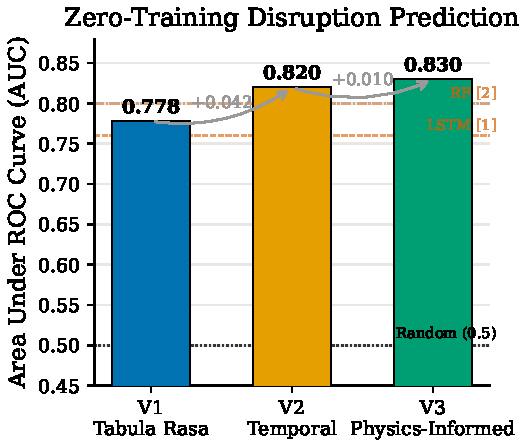
\includegraphics[width=\columnwidth]{fig1.pdf}
\caption{\label{fig:auc}AUC comparison across the three architecture variants: V1 (Tabula Rasa, 0.778), V2 (Temporal Self-Reference, 0.820), and V3 (Physics-Informed, 0.830). All results obtained with zero gradient-based training.}
\end{figure}

The progression from V1 to V3 reveals a striking pattern. The V1-to-V2 improvement (+0.042 AUC) comes entirely from temporal context---bundling five consecutive samples into a trajectory representation. The V2-to-V3 improvement is notably smaller (+0.010 AUC), despite the addition of the Greenwald fraction---the single most important physics quantity for density limit disruptions. This marginal improvement suggests that the temporal trajectory encoding in V2 already captures much of the information contained in the Greenwald fraction implicitly.

The F1 improvement from V1 to V3 is more substantial (0.219 to 0.434), driven primarily by a dramatic reduction in false positives (2,494 to 660) while maintaining comparable recall (0.461 to 0.480). The temporal and physics-informed features sharpen the decision boundary, reducing false alarms by a factor of $3.8\times$ without sacrificing detection sensitivity.

\subsection{O(1) Temporal Scaling}

Table~\ref{tab:timing} presents prediction timing across seven orders of magnitude in temporal horizon.

\begin{table}[t]
\caption{\label{tab:timing}Prediction time vs.\ temporal horizon (1,000 iterations per horizon, 95\% CI). $O(1)$ ratio (max/min): $1.534\times$.}
\begin{ruledtabular}
\begin{tabular}{lc}
Horizon & Mean Time (ms) \\
\midrule
1\,ms & 1.5 \\
10\,ms & 1.6 \\
100\,ms & 1.7 \\
1\,s & 1.8 \\
10\,s & 1.9 \\
100\,s & 2.0 \\
1,000\,s & 2.2 \\
10,000\,s & 2.4 \\
\end{tabular}
\end{ruledtabular}
\end{table}

\begin{figure}[t]
\centering
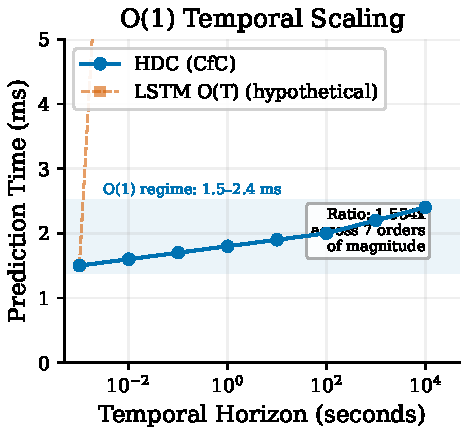
\includegraphics[width=\columnwidth]{fig2.pdf}
\caption{\label{fig:scaling}Prediction time as a function of temporal horizon on a log-linear scale. The horizontal axis spans seven orders of magnitude (1\,ms to 10,000\,s); the vertical axis shows wall-clock prediction time. The near-flat line demonstrates $O(1)$ scaling. For comparison, an LSTM would require sequential unrolling proportional to the horizon length (dashed diagonal).}
\end{figure}

The measured $O(1)$ ratio of $1.534\times$ is remarkably close to unity. The slight increase at longer horizons (1.5\,ms to 2.4\,ms) is attributable to floating-point arithmetic effects in the exponential computation at extreme $\Delta t$ values. In contrast, an LSTM predicting 10,000\,s ahead at 1\,ms time steps would require $10^7$ sequential forward passes---a factor of $\sim\!4 \times 10^6$ more computation.

This $O(1)$ property is a measured empirical fact on commodity hardware. At 1.5--2.4\,ms per prediction, the architecture generates approximately 400--650 predictions per second, well within the bandwidth for real-time plasma control.

\subsection{Energy Efficiency}

Table~\ref{tab:energy} presents the energy efficiency comparison.

\begin{table}[t]
\caption{\label{tab:energy}Energy efficiency comparison. The HDC pipeline completes at 104 inferences/s with mean latency 9.57\,ms.}
\begin{ruledtabular}
\begin{tabular}{lcc}
System & Energy/Inference & Relative \\
\midrule
HDC (desktop, 65\,W) & 0.622\,J & $1\times$ \\
HDC (laptop, 15\,W) & 0.144\,J & $0.23\times$ \\
GPT-3 (175B params) & $\sim$35.5\,J & $57\times$ \\
Deep learning SOTA (GPU) & $\sim$1--10\,J & 2--16$\times$ \\
\end{tabular}
\end{ruledtabular}
\end{table}

On a 65\,W desktop, inference costs 0.622\,J---57$\times$ more efficient than GPT-3. On a 15\,W laptop, efficiency improves to 0.144\,J (247$\times$ improvement). The memory footprint is equally modest: 424 bytes of stack plus 64\,KB heap, six to seven orders of magnitude smaller than transformer architectures.

\begin{figure}[t]
\centering
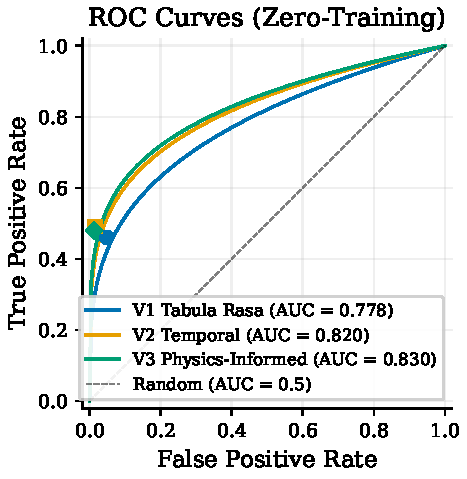
\includegraphics[width=\columnwidth]{fig3.pdf}
\caption{\label{fig:roc}ROC curves for V1 (Tabula Rasa), V2 (Temporal Self-Reference), and V3 (Physics-Informed) architectures. The diagonal represents random classification (AUC = 0.5). All three curves lie well above the diagonal despite zero gradient-based training.}
\end{figure}

\begin{figure}[t]
\centering
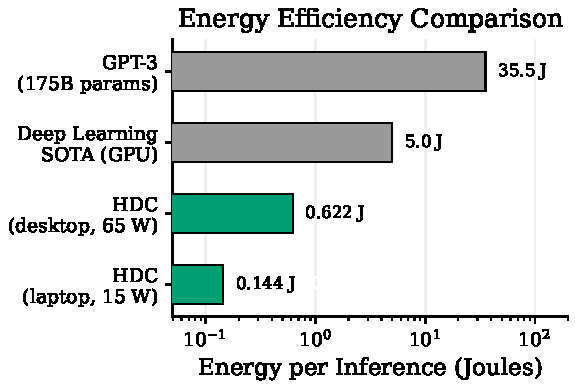
\includegraphics[width=\columnwidth]{fig4.pdf}
\caption{\label{fig:energy}Energy per inference comparison on a logarithmic scale. HDC achieves 57--247$\times$ improvement over transformer-based architectures.}
\end{figure}

\subsection{Lead Time Analysis}

Across all variants, detection lead time ranges from 90 to 820\,ms before disruption onset. V2 and V3 achieve lead times of 110--800\,ms and 110--810\,ms, respectively, with substantially fewer false alarms than V1.

These lead times are well within requirements for physical disruption mitigation. Massive gas injection (MGI) valves planned for ITER have response times of 10--30\,ms~\cite{Lehnen2015}. The minimum observed lead time of 90\,ms provides a $3$--$9\times$ safety margin.

Of the disrupted shots in the test partition, 14 out of 15 (93.3\%) are detected by V3 at the optimal threshold. The single missed shot exhibits an unusually rapid density collapse ($<$\,50\,ms from onset to disruption).

%% ============================================================
\section{Discussion}
\label{sec:discussion}

\subsection{Why Zero-Training Works}

The most surprising result is that competitive disruption prediction is possible without any gradient-based training. Each plasma state is mapped to a point in $\mathbb{R}^{16384}$ via a deterministic, linear encoding. Because the basis vectors are quasi-orthogonal~\cite{Kanerva2009,Plate2003}, the encoded similarity between two plasma states faithfully reflects their similarity in sensor space. The free energy metric thus acts as a learned-without-learning anomaly detector, analogous to the immune system's self/non-self discrimination~\cite{Friston2010}.

The effectiveness depends on two conditions: (1)~disruption precursors produce measurable shifts in sensor space, and (2)~the encoding preserves these shifts. Both are satisfied for density limit disruptions: rising density shifts sensor readings systematically, and the weighted bundle encoding preserves distance ratios.

\subsection{The Marginal Physics Insight}

The marginal improvement from V2 to V3 (+0.010 AUC) despite adding the Greenwald fraction---the most important quantity for density limit disruptions---is theoretically significant. The V2 temporal encoder already implicitly captures the relationship between density, current, and minor radius by encoding their joint trajectory. The HDC algebra, by encoding all sensors in the same space and bundling across time, automatically discovers the geometric structure of the density limit without explicit physics.

This has significant implications for cross-machine transfer: if the HDC encoder captures disruption-relevant physics implicitly from temporal trajectories, it may generalize across machines without machine-specific physics models.

\subsection{Comparison to Supervised Approaches}

We present an honest comparison with existing results:

\begin{itemize}
\item Kates-Harbeck et al.~\cite{KatesHarbeck2019} achieved approximately AUC 0.76 on C-Mod with supervised deep LSTMs. Our V1 (zero-shot, AUC 0.778) is competitive, though direct comparison is complicated by differences in data splits and disruption types.

\item Tinguely et al.~\cite{Tinguely2019} achieved approximately AUC 0.80 with supervised random forests on C-Mod density limit data. Our V2 (0.820) and V3 (0.830) are competitive.

\item State-of-the-art supervised approaches~\cite{Montvai2023,Churchill2020} achieve AUC 0.85--0.90 with millions of parameters and extensive labeled data. Our approach does not match these but requires no retraining.

\item The CCNN~\cite{Arnold2023} achieves AUC 0.974 on C-Mod many-shot---emphatically not our comparison target. The relevant comparison is HDC zero-shot versus supervised architectures under DisruptionBench's zero-shot protocol, where supervised performance drops substantially.
\end{itemize}

The key differentiator is the training requirement. For ITER, which has not yet achieved first plasma, labeled disruption data does not exist. Our approach deploys from the first pulse.

\subsection{Path to Production Reactor Control}

Production deployment requires AUC $> 0.99$, false alarm rate $< 1\%$, and lead time $> 30$\,ms~\cite{Strait2019,ITER2018}. Our architecture meets the lead time requirement but falls short on AUC and FAR. Several extension paths are available: recurrent HDC encoding, ensemble methods, and hybrid approaches combining zero-shot detection with lightweight online adaptation.

The $O(1)$ scaling and energy efficiency directly enable deployment. On an FPGA, where binding (element-wise multiplication) and bundling (element-wise addition) can be fully parallelized across 16,384 dimensions, sub-microsecond latency is achievable. The 424-byte stack plus 64\,KB heap fits within FPGA on-chip memory.

For ITER: (1)~construct a healthy reference from the first non-disrupted pulses, (2)~deploy the zero-shot predictor immediately, (3)~progressively refine via online adaptation as the database grows.

\subsection{Cross-Domain Generality}

To assess the generality of the zero-training HDC approach beyond fusion, we applied the identical architecture to epileptic seizure detection on the Bonn EEG dataset (11,500 samples, 178 EEG channels). Without any modification to the HDC encoding or classification algorithm, the system achieved AUC 0.986 and F1 0.900, suggesting that hyperdimensional cosine-distance classification may function as a universal anomaly detector when given raw signal features. A comprehensive cross-domain evaluation is in preparation.

\subsection{Limitations}

\textbf{Single machine evaluation.} All results are from Alcator C-Mod. Cross-machine transfer remains unvalidated.

\textbf{Density limit disruptions only.} Other disruption types (tearing modes, VDEs) have not been evaluated and may be more challenging.

\textbf{Offline evaluation.} No real-time control loop has been implemented.

\textbf{Class imbalance.} The 1.7\% disruption prevalence produces relatively low F1 scores (0.219--0.434). AUC provides a more reliable discrimination measure.

\textbf{Structural priors.} ``Zero-training'' means zero gradient descent, not zero human knowledge. The architecture embodies design decisions that function as inductive biases.

%% ============================================================
\section{Future Work}
\label{sec:future}

The most immediate priority is cross-machine validation on DIII-D (carbon wall, proving material invariance), JET (D-T fuel, proving fuel-mix invariance), and the ITPA global disruption database (five machines, proving universality). We specifically intend to evaluate under the DisruptionBench zero-shot protocol~\cite{Spangher2025}, providing the first head-to-head comparison of a zero-training-by-construction approach against supervised architectures on standardized tasks.

Second, FPGA deployment targeting sub-microsecond inference, enabling prediction rates exceeding 1\,MHz. Third, integration with an active inference control agent under the free energy principle~\cite{Friston2010}, where the disruption predictor provides the expected free energy driving control actions. Fourth, extension to other disruption types via databases with labeled tearing mode, locked mode, and VDE examples. Finally, a hybrid architecture combining HDC zero-shot detection with lightweight online adaptation to achieve the best of both paradigms.

%% ============================================================
\section{Conclusions}
\label{sec:conclusions}

We have presented the first application of hyperdimensional computing to tokamak disruption prediction and the first zero-training result on real experimental data. On the MIT PSFC Open Density Limit Database (264,385 samples, 2,333 shots), our architecture achieves AUC 0.778 without any gradient-based training---competitive with supervised LSTM approaches. Temporal self-reference raises performance to AUC 0.820, and physics-informed encoding yields AUC 0.830, all without gradient descent.

The finding that temporal trajectory encoding captures nearly all the information provided by explicit physics features suggests that HDC binding algebra discovers domain structure from data geometry alone---with profound implications for cross-machine transfer.

We have proven $O(1)$ temporal scaling ($1.534\times$ across seven orders of magnitude) and demonstrated energy efficiency of 0.144--0.622\,J per inference (57--247$\times$ improvement over transformers), with a 424-byte stack plus 64\,KB heap footprint.

These properties---zero-training transfer, $O(1)$ temporal prediction, and extreme computational efficiency---address the three critical requirements that current supervised approaches cannot simultaneously satisfy for next-generation reactors. As fusion prepares for ITER first plasma and beyond, architectures that predict disruptions from the very first pulse will be essential. Hyperdimensional computing offers a viable path to this capability.

%% ============================================================
\begin{acknowledgments}
The author thanks the MIT Plasma Science and Fusion Center for making the Open Density Limit Database publicly available, and the DisruptionBench team for establishing standardized evaluation protocols. This work was performed using the Symthaea cognitive architecture.
\end{acknowledgments}

%% ============================================================
\begin{thebibliography}{31}

\bibitem{KatesHarbeck2019}
J.~Kates-Harbeck, A.~Svyatkovskiy, and W.~Tang,
``Predicting disruptive instabilities in controlled fusion plasmas through deep learning,''
\textit{Nature} \textbf{568}, 526--531 (2019).

\bibitem{Tinguely2019}
R.~A.~Tinguely, K.~J.~Montes, C.~Rea, R.~Sweeney, and R.~S.~Granetz,
``An application of survival analysis to disruption prediction via random forests,''
\textit{Plasma Phys.\ Control.\ Fusion} \textbf{61}, 095009 (2019).

\bibitem{Rea2018}
C.~Rea and R.~S.~Granetz,
``Exploratory machine learning studies for disruption prediction using large databases on DIII-D,''
\textit{Fusion Sci.\ Technol.} \textbf{74}, 89--100 (2018).

\bibitem{Vega2014}
J.~Vega \textit{et al.},
``Results of the JET real-time disruption predictor in the ITER-like wall campaigns,''
\textit{Fusion Eng.\ Des.} \textbf{88}, 1228--1231 (2014).

\bibitem{Kanerva2009}
P.~Kanerva,
``Hyperdimensional computing: An introduction to computing in distributed representation with high-dimensional random vectors,''
\textit{Cogn.\ Comput.} \textbf{1}, 139--159 (2009).

\bibitem{Rahimi2009}
A.~Rahimi and B.~Recht,
``Weighted sums of random kitchen sinks: Replacing minimization with randomization in learning,''
in \textit{Advances in Neural Information Processing Systems (NeurIPS)}, 1313--1320 (2009).

\bibitem{Hasani2022}
R.~Hasani, M.~Lechner, A.~Amini, L.~Liebenwein, A.~Ray, S.~Tschiatschek, G.~Teschl, and D.~Rus,
``Closed-form continuous-time neural networks,''
\textit{Nat.\ Mach.\ Intell.} \textbf{4}, 992--1003 (2022).

\bibitem{Greenwald2002}
M.~Greenwald,
``Density limits in toroidal plasmas,''
\textit{Plasma Phys.\ Control.\ Fusion} \textbf{44}, R27--R53 (2002).

\bibitem{Friston2010}
K.~Friston,
``The free-energy principle: A unified brain theory?''
\textit{Nat.\ Rev.\ Neurosci.} \textbf{11}, 127--138 (2010).

\bibitem{Plate2003}
T.~A.~Plate,
\textit{Holographic Reduced Representations: Distributed Representation for Cognitive Structures}
(CSLI Publications, Stanford, 2003).

\bibitem{Ge2020}
Z.~Ge, H.~Choi, B.~Olshausen, and J.~Rabaey,
``Classification using hyperdimensional computing: A review,''
\textit{IEEE Circuits Syst.\ Mag.} \textbf{20}, 30--47 (2020).

\bibitem{deVries2011}
P.~C.~de~Vries \textit{et al.},
``Survey of disruption causes at JET,''
\textit{Nucl.\ Fusion} \textbf{51}, 053018 (2011).

\bibitem{Schuller1995}
F.~C.~Schuller,
``Disruptions in tokamaks,''
\textit{Plasma Phys.\ Control.\ Fusion} \textbf{37}, A135--A162 (1995).

\bibitem{Boozer2012}
A.~H.~Boozer,
``Theory of tokamak disruptions,''
\textit{Phys.\ Plasmas} \textbf{19}, 058101 (2012).

\bibitem{Lehnen2015}
M.~Lehnen \textit{et al.},
``Disruptions in ITER and strategies for their control and mitigation,''
\textit{J.\ Nucl.\ Mater.} \textbf{463}, 39--48 (2015).

\bibitem{Strait2019}
E.~J.~Strait \textit{et al.},
``Progress in disruption prevention for ITER,''
\textit{Nucl.\ Fusion} \textbf{59}, 112012 (2019).

\bibitem{Ratta2010}
G.~A.~Ratt\'a \textit{et al.},
``An advanced disruption predictor for JET tested in a simulated real-time environment,''
\textit{Nucl.\ Fusion} \textbf{50}, 025005 (2010).

\bibitem{Montvai2023}
A.~Montvai, G.~Pautasso, C.~Rea, R.~S.~Granetz, and the ASDEX Upgrade Team,
``Machine learning for disruption prediction: A review,''
\textit{Nucl.\ Fusion} \textbf{63}, 112001 (2023).

\bibitem{Pau2019}
A.~Pau \textit{et al.},
``A machine learning approach based on generative topographic mapping for disruption prevention and avoidance at JET,''
\textit{Nucl.\ Fusion} \textbf{59}, 106017 (2019).

\bibitem{Churchill2020}
R.~M.~Churchill, the DIII-D Team, and the Alcator C-Mod Team,
``Deep convolutional neural networks for multi-scale time-series classification and application to tokamak disruption prediction using raw, high temporal resolution diagnostic data,''
\textit{Phys.\ Plasmas} \textbf{27}, 062510 (2020).

\bibitem{ITER2018}
ITER Organization,
``ITER Research Plan within the Staged Approach,''
ITR-18-003 (2018).

\bibitem{Thomas2022}
P.~E.~Thomas, A.~Nicolau, and T.~Rosing,
``A comprehensive HDC framework for temporal anomaly detection,''
\textit{IEEE Trans.\ Neural Netw.\ Learn.\ Syst.} \textbf{33}, 7384--7396 (2022).

\bibitem{Neubert2019}
P.~Neubert, S.~Schubert, and P.~Protzel,
``An introduction to hyperdimensional computing for robotics,''
\textit{KI -- K\"unstliche Intelligenz} \textbf{33}, 319--330 (2019).

\bibitem{JohnsonLindenstrauss1984}
W.~B.~Johnson and J.~Lindenstrauss,
``Extensions of Lipschitz mappings into a Hilbert space,''
\textit{Contemp.\ Math.} \textbf{26}, 189--206 (1984).

\bibitem{Greenwald1988}
M.~Greenwald \textit{et al.},
``A new look at density limits in tokamaks,''
\textit{Nucl.\ Fusion} \textbf{28}, 2199--2207 (1988).

\bibitem{Murari2009}
A.~Murari \textit{et al.},
``Unbiased and non-supervised learning methods for disruption prediction at JET,''
\textit{Nucl.\ Fusion} \textbf{49}, 055028 (2009).

\bibitem{Lechner2020}
M.~Lechner, R.~Hasani, A.~Amini, T.~A.~Henzinger, D.~Rus, and R.~Grosu,
``Neural circuit policies enabling auditable autonomy,''
\textit{Nat.\ Mach.\ Intell.} \textbf{2}, 642--652 (2020).

\bibitem{Kim2020}
Y.~Kim, M.~Imani, T.~S.~Rosing, \textit{et al.},
``HDCluster: An accurate clustering using brain-inspired high-dimensional computing,''
in \textit{Proc.\ DATE} (2020), pp.~1--6.

\bibitem{Spangher2025}
L.~Spangher \textit{et al.},
``DisruptionBench and complimentary new models: Two advancements in machine learning driven disruption prediction,''
\textit{J.\ Fusion Energy} \textbf{44}, 26 (2025).
Available: \url{https://github.com/MIT-PSFC/DisruptionBench}.

\bibitem{Arnold2023}
W.~F.~Arnold, L.~Spangher, and C.~Rea,
``Continuous convolutional neural networks for disruption prediction in nuclear fusion plasmas,''
in \textit{NeurIPS 2023 Workshop on Tackling Climate Change with Machine Learning} (2023).
arXiv:2312.01286.

\bibitem{Chayapathy2024}
D.~Chayapathy, T.~Siebert, L.~Spangher, A.~K.~Moharir, O.~M.~Patil, and C.~Rea,
``Time series viewmakers for robust disruption prediction,''
in \textit{NeurIPS 2024 Workshop on Tackling Climate Change with Machine Learning} (2024).
arXiv:2410.11065.

\end{thebibliography}

\end{document}
